% 1987 年全国卷文科第 5 题：二次函数图象
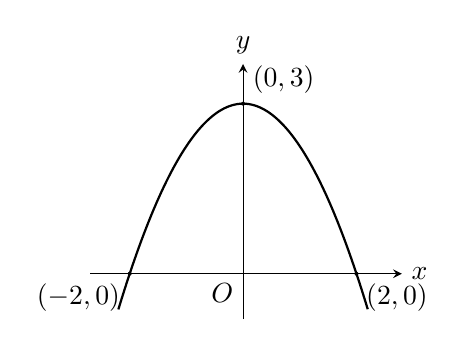
\begin{tikzpicture}[scale=0.72,>=stealth]
  \draw[->] (-2.7,0)--(2.8,0) node[right] {$x$};
  \draw[->] (0,-0.8)--(0,3.7) node[above] {$y$};
  \draw[thick,domain=-2.2:2.2,samples=100]
    plot (\x,{3-0.75*\x*\x});
  \fill (-2,0) circle (1pt) node[below left] {$(-2,0)$};
  \fill (2,0) circle (1pt) node[below right] {$(2,0)$};
  \fill (0,3) circle (1pt) node[above right] {$(0,3)$};
  \node[below left] at (0,0) {$O$};
\end{tikzpicture}
